\section{Empirical Results}

\subsection{Overview of the empirical output}
\label{sec:results_overview}

The pipeline provides a comprehensive and internally consistent set of factual data: out-of-sample metrics, model rankings, Diebold--Mariano diagnostics, classification statistics at the signal level, the forecast series themselves, and diagnostic metrics. This breadth is intentional. The empirical results are not based on a single table. Instead, the main conclusions are supported from several perspectives: average forecast accuracy, paired-loss diagnostics, error behavior over time, and the effectiveness of stress scenario warnings.

Two conclusions follow from what is stated below. First, the process of dependence can be predicted based on a sample in accordance with a strict step-by-step plan. Second, almost all of this predictability stems from the object's own stability, while functions related to various assets provide little additional predictive information. Taken together, these two conclusions describe the nature of the forecasting problem and its main limitations.

\subsection{Average dependency-forecasting performance}

Table~\ref{tab:model_ranking_summary} gives each model's average out-of-sample performance across all dependency experiments, ranked by RMSE, the metric that reacts most to the large misses that matter on a smooth, bounded target.

\begin{table}[H]
    \centering
    \caption{Average out-of-sample forecasting performance across all dependency experiments.}
    \label{tab:model_ranking_summary}
    \begin{tabular}{lrcrr}
        \toprule
        Model & Average RMSE & 95\% CI for RMSE & Average MAE & Average $R^2$ \\
        \midrule
        Ridge             & 0.0656 & [0.0611,\ 0.0701] & 0.0419 & 0.9432 \\
        AR(1)             & 0.0659 & [0.0613,\ 0.0706] & 0.0403 & 0.9424 \\
        HAR               & 0.0659 & [0.0613,\ 0.0706] & 0.0405 & 0.9424 \\
        Naive (last value) & 0.0666 & [0.0619,\ 0.0714] & 0.0395 & 0.9412 \\
        ElasticNet        & 0.0669 & [0.0625,\ 0.0713] & 0.0434 & 0.9411 \\
        Ensemble          & 0.0694 & [0.0652,\ 0.0738] & 0.0462 & 0.9365 \\
        GBM               & 0.0886 & [0.0842,\ 0.0932] & 0.0625 & 0.8983 \\
        Random Forest     & 0.0905 & [0.0860,\ 0.0952] & 0.0636 & 0.8936 \\
        XGBoost           & 0.1241 & [0.1184,\ 0.1297] & 0.0864 & 0.7923 \\
        DCC-GARCH         & 0.2136 & [0.2067,\ 0.2203] & 0.1683 & 0.3715 \\
        \bottomrule
    \end{tabular}
    \par\smallskip\noindent\footnotesize{\textit{Note: Results averaged across all asset-pair and window-length combinations. RMSE and R$^2$ computed on out-of-sample walk-forward predictions. The interval column averages the per-experiment bootstrap bounds over the same 24 experiments: for each experiment the $(y_t, \hat{y}_t)$ pairs are resampled with replacement 500 times and the 2.5th and 97.5th percentiles of the resulting RMSE distribution are taken (\texttt{07\_Robustness\_Checks.ipynb}, Appendix~\ref{app:reproducibility}). The column describes the typical width of the interval around each model's error, not a pooled confidence interval for the average itself; and because the resampling is i.i.d.\ over pairs while the forecast errors are serially correlated, the intervals are, if anything, too narrow. HAR = Heterogeneous AutoRegressive model; Ensemble = adaptive inverse-RMSE-weighted ensemble. Best-performing model by average RMSE is Ridge (regularised linear regression with StandardScaler). All metrics reflect the full sample through 16 May 2026 (3{,}053 observations).}}
\end{table}

The top three (Ridge, AR(1), and HAR) are nearly indistinguishable, with average RMSE of 0.0656, 0.0659, and 0.0659 and $R^2$ of 0.9424 and above. The 0.0003 spread between them is economically meaningless, and the naive last-value baseline sits only just outside at RMSE 0.0666, which already indicates that serial persistence accounts for most of the forecastable variation.

The bootstrap intervals put the spread in perspective. Each of the top four models carries an interval roughly 0.009 wide, against differences between them of 0.0003 to 0.0010, while nothing in the leading cluster comes within 0.01 of GBM or Random Forest and DCC-GARCH sits further away than any of these intervals is wide, by more than an order of magnitude. Overlapping marginal intervals are only suggestive, however, since the models are evaluated on the same observations and their errors are strongly correlated; the question of whether one model genuinely beats another has to be settled on the paired loss differentials.

The paired Diebold--Mariano diagnostics do not support a stable ordering at the top. Ridge, the leader on average RMSE, has a lower loss than the naive last-value baseline in 6 of the 24 experiments, a higher loss in 9, and a similar loss in the remaining 9 under the reported zero-lag DM calculation. HAR shows lower loss in 7, higher loss in 1, and similar loss in 16. Because the rolling targets overlap, these DM classifications are descriptive rather than formal significance tests; their direction nevertheless reinforces the conclusion that the ordering changes with asset pair and window length. The picture below the top tier is different: GBM, Random Forest, and XGBoost have higher RMSE than the naive baseline in all 24 experiments. What the ranking supports is a division into tiers, not an inferential ordering inside the top tier. One nuance should be stated explicitly: the ranking here is by RMSE, on which Ridge leads. On mean absolute error the ordering differs, with the naive last-value baseline formally best (MAE 0.0395), ahead of AR(1) (0.0403), HAR (0.0405), and Ridge (0.0419). RMSE penalises large errors more heavily, so Ridge effectively trades a few more small errors for fewer large ones. ElasticNet and the adaptive Ensemble form a second tier above $R^2 = 0.93$. The tree methods (GBM, Random Forest, XGBoost) trail well behind, with RMSE between roughly 0.09 and 0.12 and $R^2$ below 0.90. DCC-GARCH finishes last by a wide margin ($R^2 = 0.3715$).

The composition of the top cluster deserves a closer look. Ridge, AR(1), and HAR reach almost the same accuracy through different mechanisms: AR(1) uses a single autoregressive coefficient, HAR combines three time scales (daily, weekly, and monthly), and Ridge fits the full regularised feature set anchored by the most recent lag. They converge because each is ultimately exploiting the same property, the strong persistence of the target, and the additional structure in HAR and Ridge does not capture anything that a single lag has not already accounted for. The convergence says more about the target than about the models: the series is so strongly autoregressive that there is little else left to capture.

\subsection{Representative forecast example}

Figure~\ref{fig:sp500_forecast} shows the out-of-sample forecast panel for Bitcoin--S\&P 500 at the 30-day window. It is the natural representative case: of all the pairs, this one ties the crypto market to the broadest gauge of U.S. equity risk.

\begin{figure}[H]
    \centering
    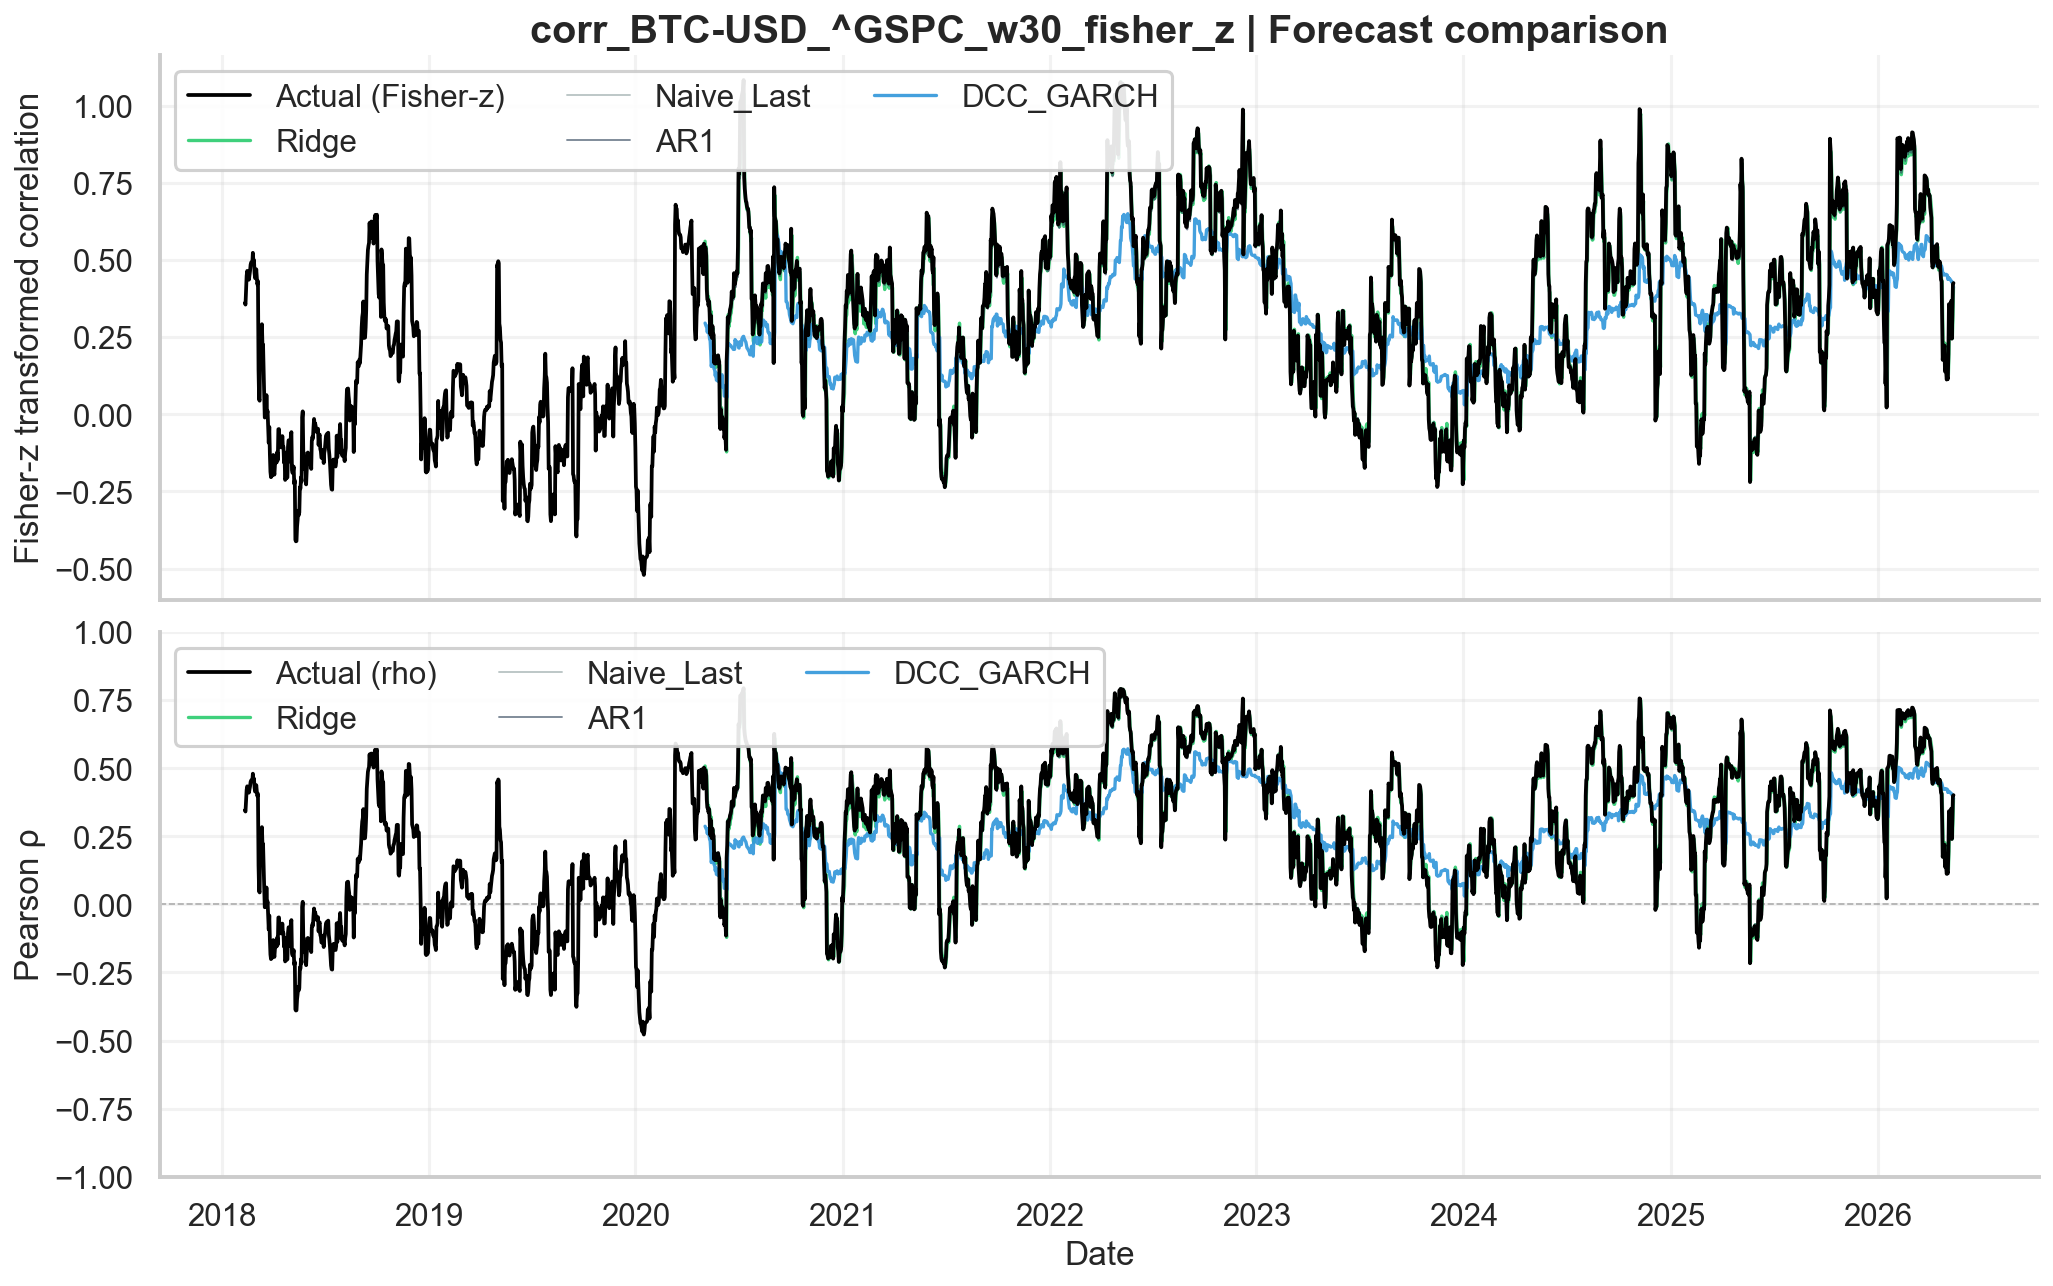
\includegraphics[width=0.95\textwidth]{../outputs/figures/thesis_forecast_corr_BTC-USD_^GSPC_w30_fisher_z.png}
    \caption{Observed and predicted Fisher-transformed dependency for the Bitcoin--S\&P 500 pair at the 30-day rolling window. Forecast series are generated under strict walk-forward evaluation with no use of future information.}
    \label{fig:sp500_forecast}
\end{figure}

The figure highlights three characteristics of the problem. First, the target moves smoothly because it is constructed using overlapping windows. Second, the best models replicate the overall trajectory with a small systematic deviation. The most challenging aspect is capturing inflection points: when the relationship changes abruptly, all models tend to respond inadequately, albeit to varying degrees. During these periods, DCC-GARCH performs the worst, while machine learning gains a relative advantage. However, it still does not outperform simple persistence in terms of overall forecasting accuracy.

\subsection{Forecasting performance by asset class}

The averages hide some useful cross-sectional variation. Bitcoin--Ethereum is the easiest pair to forecast: the two share liquidity and sentiment drivers, so their correlation is especially smooth and autocorrelated. It posts the highest out-of-sample $R^2$ of any pair, and longer windows push it higher still.

The precious-metal pairs, Bitcoin--Gold and Bitcoin--Silver, sit in the middle. Their rolling correlation is regime-dependent, drifting between near-zero and weakly positive or negative. Even so, the target stays forecastable, and persistence-based models keep the lead.

The stock index pairs—Bitcoin-S\&P 500 and Bitcoin-NASDAQ—are the most relevant in practice. They link cryptocurrency price movements to broader market risk appetite and, on average, are the most predictable among non-crypto pairs. During periods of calm, the relationship is relatively smooth and exhibits strong autocorrelation, which also favors forecasts based on stationarity. However, these pairs are also highly sensitive to changes in market conditions. Their co-movement may intensify during periods of heightened risk and can change abruptly during market turmoil. These sharp changes lead to random spikes in forecast errors that are not fully accounted for by any model, making them the primary short-term challenge for forecasting stock pairs.

The Bitcoin-Dollar Index pair exhibits the weakest and most specific correlation, as well as the lowest average predictability. Nevertheless, it has been included to test whether a set of cryptographic functions can capture the macroeconomic trend channel at all.

To check that the lower errors on equity pairs are not just luck, the pooled out-of-sample losses of the equity pairs (S\&P 500, NASDAQ) are tested against those of the non-equity pairs (gold, silver, dollar index) with a two-sample Diebold--Mariano test \cite{diebold1995}. The two groups have different targets, and therefore loss series on different scales, so this pooled comparison is descriptive; it nonetheless indicates that the equity-pair advantage is systematic.

\subsection{The persistence dominance result}

That simple persistence models lead the average ranking was to be expected.

This result follows directly from the construction of the target. A rolling Pearson correlation over $w$ calendar days shares $w-1$ observations with the previous window, which smooths the series in a way similar to a moving average. After applying the Fisher transform, the resulting series is strongly autocorrelated, and the first lag already explains most of the predictable variation. As a result, any model that relies heavily on the most recent value can achieve a high out-of-sample $R^2$ almost by construction.

The Random Forest feature importances point to the same conclusion. The lagged dependency term dominates the ranking in every experiment, while the return lags, rolling volatilities, and the regime gap contribute very little. The problem is forecastable mainly because the target is highly persistent; the features carry no strong cross-asset signal beyond what recent dependency already shows.

\subsection{Feature-group ablation}
\label{sec:ablation}

Feature importances describe how a fitted model distributes weight; they do not say what the model would have achieved without a given block of inputs. To measure that directly, the same models are retrained on a nested sequence of feature sets, from a single dependency lag up to the full matrix, under the identical walk-forward protocol, split points, and seeds. Only the columns of the design matrix change between runs. The five sets follow the order in which a practitioner would naturally build the model: the lagged target first, then everything derivable from the history of the dependency series, then the base asset's own returns, then the paired asset's, and finally the cross-asset interaction terms. Table~\ref{tab:feature_ablation} reports the result for the representative Bitcoin--S\&P 500 experiment at $w = 30$. The experiment is reproduced end to end by \texttt{run\_ablation.py} and, in annotated form, by \texttt{09\_Feature\_Ablation.ipynb} (Appendix~\ref{app:reproducibility}).

\begin{table}[H]
    \centering
    \caption{Feature-group ablation, Bitcoin--S\&P~500 at $w = 30$. Each row adds a block of features to the row above and keeps everything before it; \# is the resulting number of columns in the design matrix.}
    \label{tab:feature_ablation}
    \begin{tabular}{lrrrrrrr}
    \toprule
    Feature set & \# & \multicolumn{2}{c}{Ridge} & \multicolumn{2}{c}{Random Forest} & \multicolumn{2}{c}{XGBoost} \\
    \cmidrule(lr){3-8}
     &  & RMSE & $R^2$ & RMSE & $R^2$ & RMSE & $R^2$ \\
    \midrule
    G1 dependency lag only & 1 & 0.0899 & 0.8849 & 0.0986 & 0.8613 & 0.0980 & 0.8631 \\
    G2 $+$ dependency history & 11 & 0.0649 & 0.9400 & 0.0884 & 0.8886 & 0.1030 & 0.8488 \\
    G3 $+$ Bitcoin returns & 20 & 0.0649 & 0.9399 & 0.0891 & 0.8868 & 0.1058 & 0.8406 \\
    G4 $+$ related-asset returns & 29 & 0.0650 & 0.9397 & 0.0902 & 0.8841 & 0.1078 & 0.8345 \\
    G5 full model & 32 & 0.0651 & 0.9397 & 0.0910 & 0.8821 & 0.1134 & 0.8166 \\
    \bottomrule
\end{tabular}

    \par\smallskip\noindent\footnotesize{\textit{Note: G2 adds the remaining dependency lags, the 5- and 20-day dependency momentum, the 252-day regime z-score, and the multi-scale correlation terms. G3 adds Bitcoin's return lags, rolling volatilities, mean return, and squared return; G4 adds the same block for the S\&P~500; G5 adds the volatility ratio and the two absolute-spread terms, which are the only features that combine both assets. Walk-forward settings are those of the main experiment ($\mathrm{min\_train} = 800$, refit every 20 steps, seed 42).}}
\end{table}

Three things follow from the table, and the third is the one worth pausing on.

The first is that the single dependency lag already delivers $R^2 = 0.885$ for Ridge. One column, no cross-asset information of any kind, and most of the forecastable variation is already accounted for.

The second conclusion is that the only functional block that leads to a significant improvement is the model's own history of dependencies. The RMSE drops from 0.0899 to 0.0649 when additional lags, impulse conditions, and the z-score of the mode are added, after which the improvement stops. If we sum the returns on Bitcoin, the RMSE is 0.0649; if we sum the returns on the S\&P 500, it is 0.0650; and if we add the conditions of interaction between assets, it is 0.0651. Starting with G2, approximately two-thirds of the design matrix does not contribute significant improvements. This is the result of constancy in its most obvious form: functions related to various assets provide little, if any, additional predictive information for the linear model.

The third conclusion is that, for tree-based ensembles, additional features are not only unhelpful but actually harmful, with performance deteriorating as new features are added. XGBoost performs best with a one-lag specification (RMSE 0.0980), and its RMSE increases with each subsequent step, rising by 16\% with the full feature set (0.1134). Random Forest improves after the dependency history is added, but its performance then also deteriorates as additional feature blocks are included. Each additional feature block expands the range of splits that the ensemble can fit. Since the added variables contain little information about the target, this additional flexibility is mainly used to fit noise within the training window. This pattern also explains a result that might otherwise seem unusual in Table (tab): tree-based methods lag behind linear models not because they are poorly suited to the target, but because they are given predictors that only a strongly regularised estimator can safely ignore.

\subsection{Comparison with DCC-GARCH}

Even though persistence baselines win the unconditional ranking, machine-learning models have lower RMSE than DCC-GARCH by a large descriptive margin. Figure~\ref{fig:dm_heatmap} shows the Diebold--Mariano diagnostic between the best machine-learning model and the DCC benchmark across every experiment.

\begin{figure}[H]
    \centering
    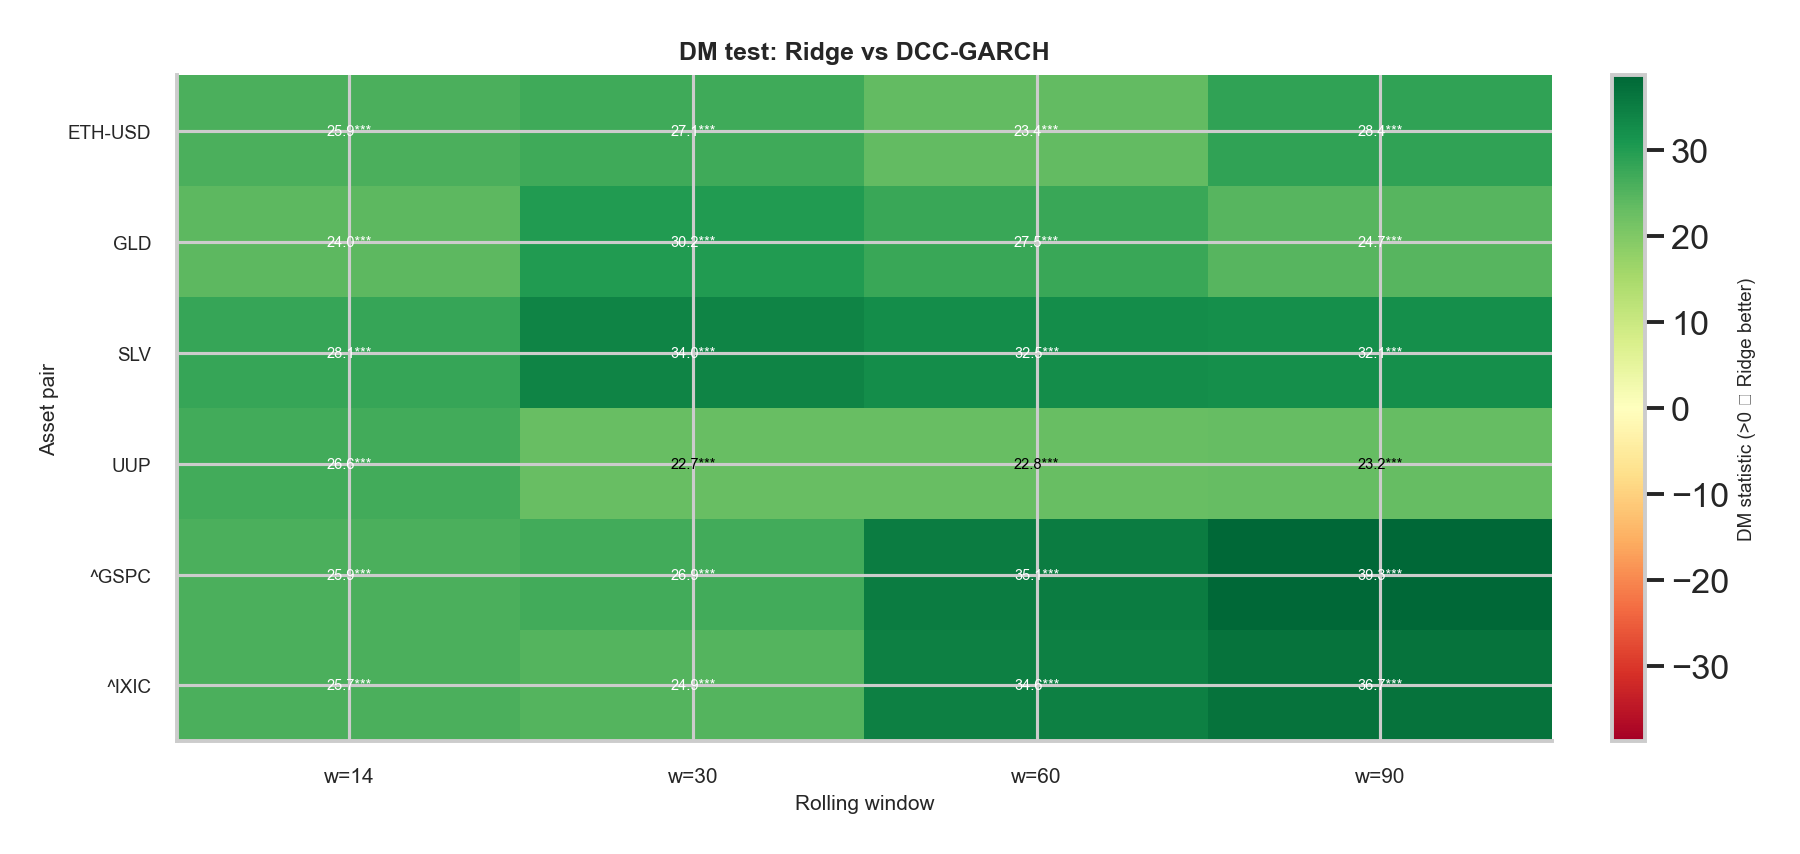
\includegraphics[width=0.82\textwidth]{../outputs/figures/dm_heatmap_Ridge_vs_DCC.png}
    \caption{Diebold--Mariano diagnostic comparing Ridge (best overall RMSE across all models) against DCC-GARCH across all asset-pair and window-length combinations. Darker cells indicate a larger positive loss-differential statistic; they do not establish formal significance because the reported standard errors use zero HAC lags.}
    \label{fig:dm_heatmap}
\end{figure}

The DM statistics are positive in every reported experiment, consistent with the lower RMSE of the best machine-learning model relative to DCC-GARCH. They are descriptive rather than confirmatory because the reported zero-lag HAC standard errors do not model autocorrelation introduced by the overlapping rolling target. The pattern has a structural explanation: DCC-GARCH is designed to model the conditional covariance of the return series, whereas the rolling Pearson correlation is a smoothed by-product of this covariance and is not targeted directly by DCC-GARCH. In contrast, the machine-learning models are trained directly on the Fisher-transformed correlation target. Thus, they are trained on the same quantity on which they are evaluated, which gives them an advantage.

This comparison involves a measurement mismatch that should be acknowledged. The rolling Pearson target is smoothed and backward-looking, with persistence created by the overlapping windows. DCC-GARCH models the instantaneous conditional covariance as a parametric and forward-looking object, so mapping its output into the rolling Pearson space introduces a systematic lag. This lag follows from the different definitions of the two objects \cite{engle2001theoretical,andersen2003realized}. The comparison remains valid because both are legitimate measures of dependence, but the size of the gap should be interpreted with caution. It should not be taken as a general verdict against DCC-GARCH.

Throughout, the thesis distinguishes two claims: benchmark superiority, meaning improvement over DCC-GARCH, and unconditional superiority, meaning improvement over AR(1). Machine learning achieves the first consistently and the second not at all. Together the two results mark out what machine learning contributes in this setting.

\subsection{Error-profile diagnostics}

Averages alone do not show when and how a model fails; that requires examining the error over time and across its distribution. Figure~\ref{fig:rolling_rmse} plots the rolling RMSE for the representative Bitcoin--S\&P 500 experiment.

\begin{figure}[H]
    \centering
    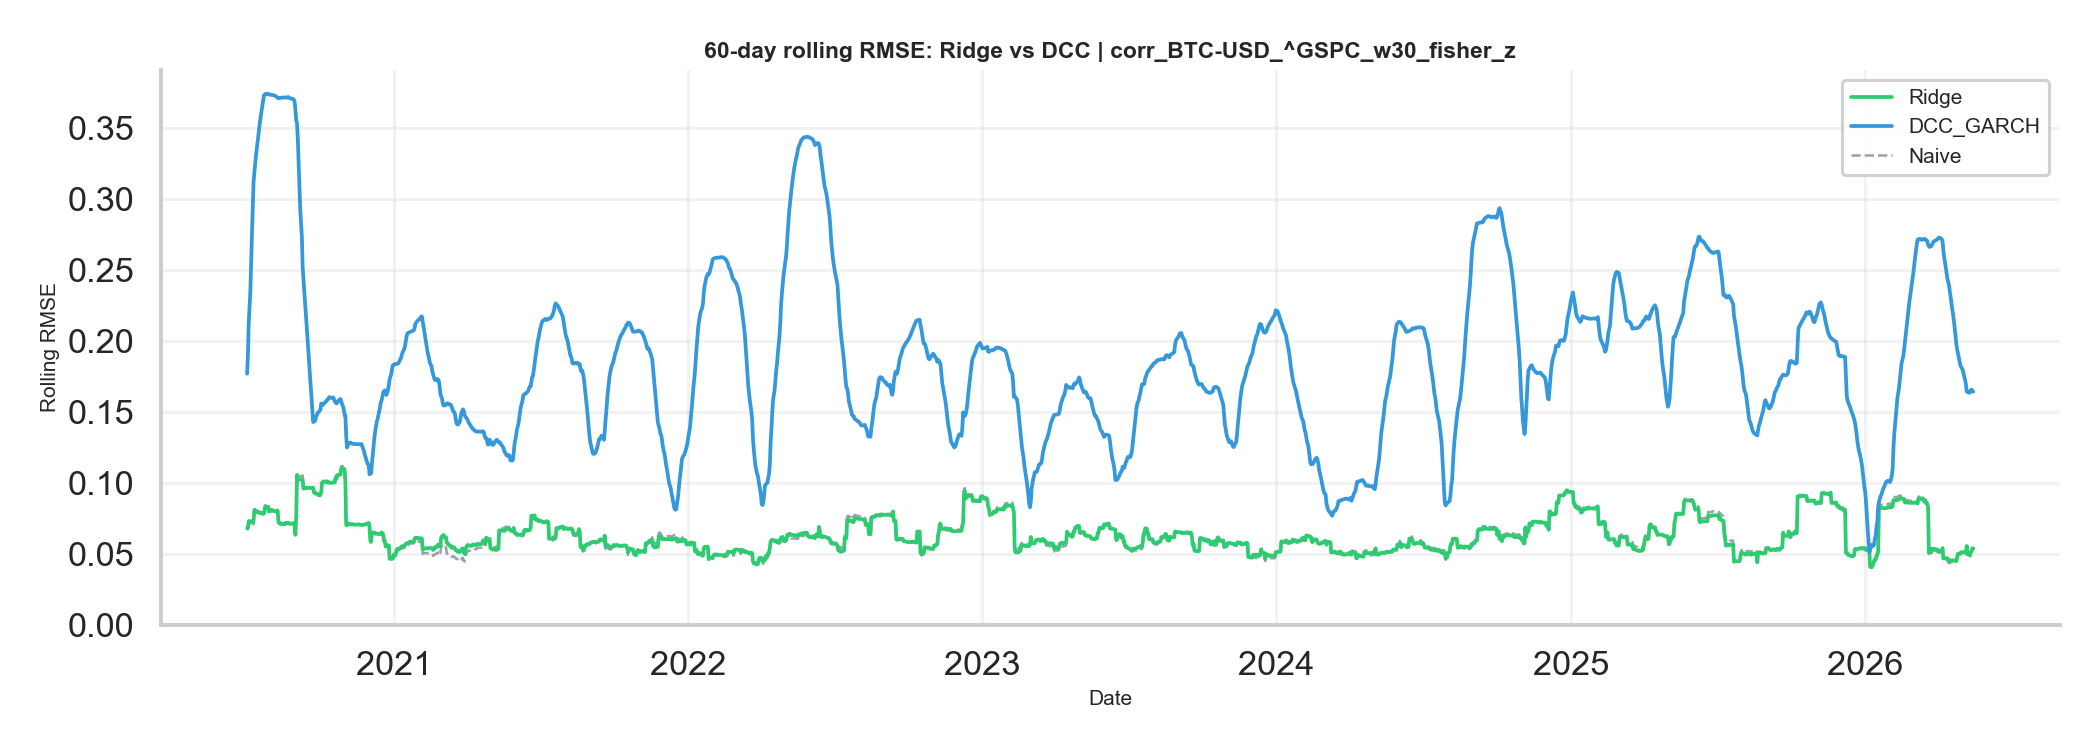
\includegraphics[width=0.9\textwidth]{../outputs/figures/rolling_rmse_corr_BTC-USD_^GSPC_w30_fisher_z.png}
    \caption{Rolling out-of-sample RMSE over time for the Bitcoin--S\&P~500 dependency experiment at the 30-day correlation window ($w=30$); the error is smoothed over a trailing 60-day window. The machine-learning model shown is Ridge, which has the lowest average RMSE overall (Table~\ref{tab:model_ranking_summary}), compared against the DCC-GARCH benchmark. Elevated error episodes correspond to periods of abrupt regime transition in the dependency process.}
    \label{fig:rolling_rmse}
\end{figure}

The quality of forecasts is far from constant over time. When the underlying relationship changes gradually, all models perform well, since it is relatively easy to capture a stable pattern. When conditions change abruptly, errors increase in all models, but to varying degrees and over different time periods. Machine learning models generally recover somewhat faster, which is consistent with their greater flexibility to relearn the relationship between features and the target after structural changes.

The error distribution confirms that the largest errors arise from episodic underreaction at sharp turning points; there is no systematic bias. The models track the slow, persistent component of the dependency reliably and perform worst on the fast, discontinuous component. This asymmetry is directly relevant to the signal layer, whose purpose is to detect the onset of stress in time.

To make this regime-sensitivity concrete, Appendix~\ref{app:market_events} summarises eleven landmark events from 2020 to 2026 on a master timeline and a correlation regime map, and provides four-panel diagnostics for four representative episodes: the COVID crash of March 2020, the FTX collapse of November 2022, the SVB banking crisis of March 2023, and the tariff shock of April 2025. Each diagnostic shows how the rolling Bitcoin correlation moved around the event relative to its pre-event baseline. The case studies are consistent with the main finding: the largest errors in Figure~\ref{fig:rolling_rmse} coincide with the sharpest events in the record.

\subsection{Investor signal layer: average results}

The second layer turns the dependency forecast into a stress-warning classifier. Table~\ref{tab:signal_summary} reports each classifier family's average performance across all asset pairs and windows.

\begin{table}[H]
    \centering
    \caption{Average investor-signal performance by classifier family, aggregated across all experiments.}
    \label{tab:signal_summary}
    \begin{tabular}{lrrr}
        \toprule
        Signal model & Balanced Accuracy & F1\_down & AUC \\
        \midrule
        Logistic regression    & 0.511 & 0.214 & 0.513 \\
        GBM (classifier)       & 0.508 & 0.158 & 0.517 \\
        Random Forest (classifier) & 0.502 & 0.042 & 0.519 \\
        \bottomrule
    \end{tabular}
    \par\smallskip\noindent\footnotesize{\textit{Note: Results averaged across all asset pairs and window lengths. Balanced Accuracy corrects for class imbalance. F1\textsubscript{down} measures detection quality for the stress class only.}}
\end{table}

Classification is a substantially harder problem than the regression layer. Stress days are noisy, rare, and asymmetrically costly to miss. The logistic classifier achieves the highest F1 on the stress class (0.214 on average), which indicates that it remains sensitive to genuine stress without collapsing into an inactive, low-exit-rate state. GBM reaches a similar balanced accuracy (0.508) but a lower F1 (0.158), because it concentrates its probability mass and triggers less often. Random Forest performs poorly, with an F1 of 0.042. Its predicted probabilities concentrate in a narrow band, so it rarely crosses the decision threshold and provides little practical value despite a comparatively high AUC.

This degenerate behaviour merits closer examination. Two factors combine to produce it: the severe imbalance between stress and non-stress days, and the absence of probability calibration. Ensemble methods are well known to produce poorly calibrated probabilities unless they are post-processed with Platt scaling \cite{platt1999probabilistic} or isotonic regression \cite{niculescu2005predicting}. GBM, which concentrates its probability mass less severely, retains a modest but non-trivial F1 (0.158). Calibration should therefore precede threshold-based signal extraction. It is not applied anywhere in the results reported here, and integrating it into the pipeline is left for future work; the Random Forest figures in particular should be read as the performance of an uncalibrated classifier rather than as evidence that the method is unsuited to the task.

This result is not surprising. In a setting with a weak signal relative to noise and correlated predictors, a regularised linear boundary can generalise better out of sample than a high-capacity ensemble, whose greater flexibility can increase variance. This is especially relevant when the data are noisy and the predictors are highly correlated.

\subsection{Best signal configurations}

The highest logistic-regression balanced accuracy occurs for Bitcoin versus the S\&P 500 at the 30-day window (0.5308; downside-class F1 = 0.2430). This is only 0.0308 above the uninformative benchmark of 0.50 and is the maximum among twenty asset-window configurations. Since no hypothesis was prespecified and no multiple-comparison correction was applied, it is a descriptive maximum rather than evidence of a reliable advantage. The signal results are therefore reported as exploratory: they motivate further validation on an untouched period, but do not establish a usable performance edge at this configuration.

Figure~\ref{fig:signal_sp500} presents the signal output for this configuration, illustrating the temporal distribution of predicted stress flags relative to realised stress events.

\begin{figure}[H]
    \centering
    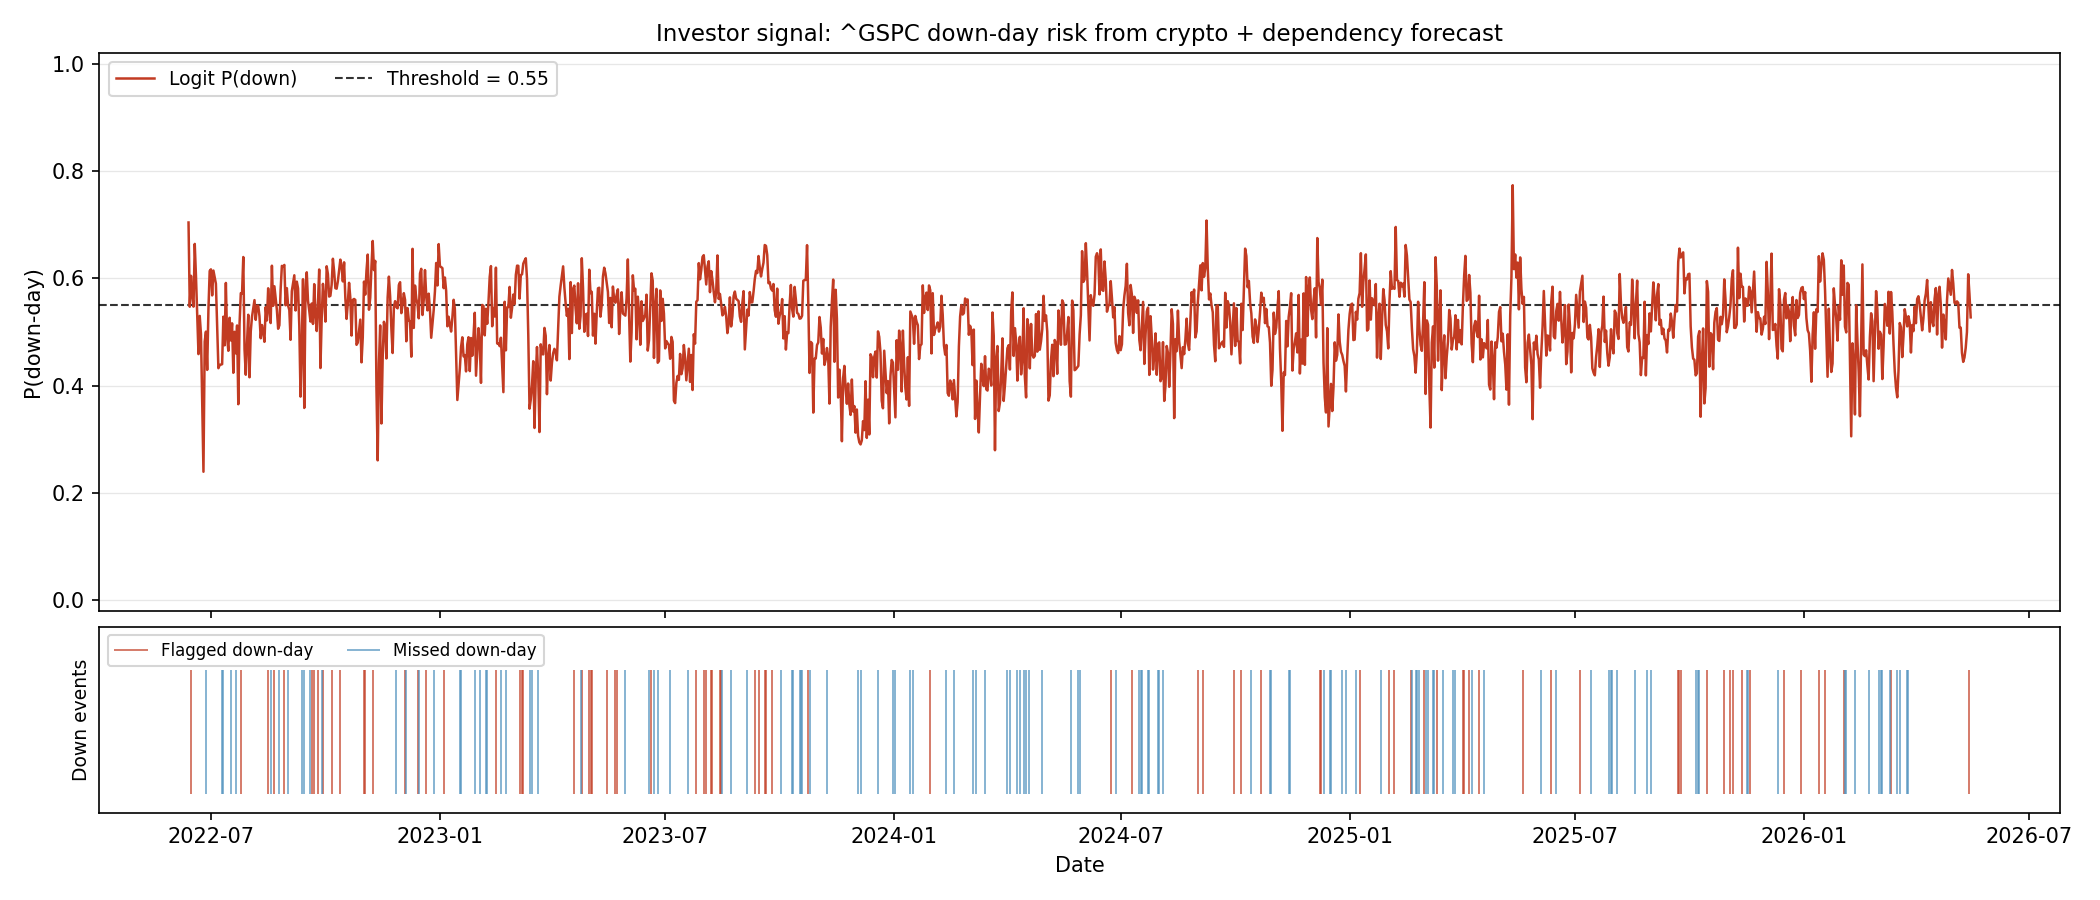
\includegraphics[width=0.95\textwidth]{../outputs/figures/signal_corr_BTC-USD_^GSPC_w30.png}
    \caption{Investor stress-warning signal for the Bitcoin--S\&P 500 pair at the 30-day window. The upper panel displays the predicted stress probability from the logistic classifier together with the decision threshold; the lower panel marks flagged and missed stress events.}
    \label{fig:signal_sp500}
\end{figure}

This signal is intended to provide probability-based warnings that identify periods of elevated risk and support risk-mitigation decisions. It is not a rule for directional trading. For the NASDAQ, the signal is noticeably weaker. The Logit balance accuracy for Bitcoin-NASDAQ falls below 0.50 in the two longer intervals, 60 and 90 days, and averages 0.4997 across all four intervals, which is the lowest result at the signal level. This difference relative to the S\&P 500 is economically justified, as the NASDAQ Composite is heavily weighted toward growth-sensitive technology stocks, whose volatility may be less closely tied to global risk appetite than that of the broader index. For precious metals and dollar-dependent currencies, the results are mixed but generally more likely to hold over short periods. This is consistent with the view that cryptocurrency movements contain some information about tensions in these markets, although the predictive signal is weaker.

\subsection{Practical interpretation of signal-layer performance}

The usefulness of the signal can only be assessed relative to a stated decision rule. An investor would consult it selectively, as one input to a conditional decision: whether to reduce exposure, tighten stops, or increase hedging when the stress probability rises.

The exit rate (how often the signal is active) is then as important as accuracy. A signal that never activates is useless whatever its nominal accuracy; one that activates constantly raises trading costs and stops carrying information. The logistic model sits between these extremes, active on roughly a fifth to a third of days depending on the pair (Table~\ref{tab:signal_returns}).

The most direct test of practical value compares the conventional asset's next-day return on days the signal flags as stress against days it leaves clear. Table~\ref{tab:signal_returns} reports this for the logistic signal, averaged across the four window lengths.

\begin{table}[H]
    \centering
    \caption{Average next-day return of the conventional asset on days flagged by the logistic signal versus days left clear, by asset pair (Logit, averaged over the four windows). Returns are in basis points per day; a positive difference means flagged days are, on average, worse. The flag rate is the share of days on which the signal is active.}
    \label{tab:signal_returns}
    \begin{tabular}{lrrrr}
        \toprule
        Asset pair & Flagged (bp) & Clear (bp) & Difference & Flag rate (\%) \\
        \midrule
        BTC--S\&P 500  & 4.08 & 5.05 & $+0.96$ & 33.1 \\
        BTC--NASDAQ    & 4.70 & 6.64 & $+1.94$ & 32.0 \\
        BTC--Gold      & 7.01 & 7.10 & $+0.08$ & 20.1 \\
        BTC--Silver    & 10.23 & 10.13 & $-0.10$ & 26.4 \\
        BTC--USD index & 0.57 & 0.89 & $+0.32$ & 31.4 \\
        \bottomrule
    \end{tabular}
\end{table}

This pattern is confirmed by the classification results. For the two equity pairs, the average next-day return is lower on flagged days than on clear days, by about 1.9 basis points per day for the NASDAQ and 1.0 basis point for the S\&P 500. This means that the signal shifts exposure away from relatively worse days, which is its intended use. For gold and silver, the difference is negligible or slightly negative, which is consistent with the weak classification performance for these pairs.

The Dollar Index is a case apart. Its absolute difference is small, at $+0.32$ basis points, but the average daily return of the series itself is also very small. In relative terms, this makes the gap between flagged and clear days the largest in the table. Given how weakly the classifier performs on this pair, this result is better read as a small-denominator artifact than as evidence of a useful signal.

Two further points are important. First, the average flagged-day return is still positive because the sample period is predominantly a rising market. The signal therefore reduces exposure to relatively worse days rather than predicting outright losses. Second, these figures are before transaction costs, which a turnover of roughly one third of days could erode. Overall, the signal works as a modest risk-reduction overlay for broad-equity exposure, but it is not strong enough to stand alone as a timing rule.

\subsection{Sensitivity to rolling window length}
\label{sec:window_sensitivity}

Window length is a first-order choice, and it visibly shapes both the target and the results. Short windows give responsive but noisy estimates; long windows give smooth, heavily autocorrelated targets that are easier to forecast but slower to register a real structural change.

The experiments identify the medium windows, and $w = 30$ days in particular, as the most useful compromise: smooth enough for high out-of-sample $R^2$ while still registering stress episodes without much delay. At longer windows the persistence effect strengthens further, narrowing the gap between the simple baselines and the complex models. This interaction between window length and model performance is itself a structural finding and a useful guide for selecting the horizon in future work.

\subsection{Summary of empirical findings}

The empirical results of the thesis are summarised in four principal statements:

\begin{enumerate}
\item Time-varying intermarket dependency between Bitcoin and conventional assets is forecastable in an out-of-sample walk-forward framework, with high average $R^2$ across every model class except the DCC-GARCH benchmark.
    \item The dominant source of predictive power is the serial persistence of the rolling correlation target; Ridge, AR(1), and HAR sit at the top with practically identical accuracy, all exploiting this persistence, while tree-based methods trail substantially.
    \item Machine-learning models have lower RMSE than the leakage-safe DCC-GARCH benchmark on the smoothed rolling-correlation target; Ridge achieves the best overall average RMSE (0.0656) across all 24 experiments. Because the reported DM standard errors do not accommodate dependence induced by the overlapping target, this is a descriptive performance comparison rather than a formal significance claim. As the discussion of this benchmark in Chapter~\ref{sec:discussion} stresses, the comparison is structurally tilted toward the ML models, since the target is a smoothed rolling correlation while DCC-GARCH estimates the instantaneous conditional correlation.
    \item The investor signal layer delivers modest classification results (on average slightly above chance, though not subjected to a formal significance test), strongest for broad equity markets. It is a supplementary risk-management input, not a self-contained directional predictor.
\end{enumerate}

These findings are consistent with one another and, together, enough to carry both the scientific and the applied contributions of the thesis. The next section takes up what they mean more broadly.

The evidence gives a consistent picture of how crypto information enters conventional-asset risk. The relationship is real and measurable, but most of the predictive information comes from the persistence of the dependency series itself. The nonlinear ability of gradient-boosted and random-forest models adds little in this setting. The dependency changes slowly over time and is sensitive to different market conditions, so simple, low-complexity models work better than more flexible, high-capacity ones. Chapter~\ref{sec:discussion} develops this interpretation and places it in the wider literature on intermarket contagion and financial machine learning.
